\section{Probabilistic Analysis} \label{s:bism}
There has been also a line of work focusing primarily on the precedence constraint, by studying the single machine case and its special instances. The scheduling problem $1|prec|\sum_jw_jC_j$ is NP-hard and many 2-approximation algorithms exists, such as \cite{hall1997scheduling}. The approximation front tops the limit since \cite{ambuhl2007inapproximability} showed that PTAS does not exist, assuming NP-complete problems cannot be solved in randomized subexponential time; and \cite{bansal2009optimal} showed that it is NP-hard to compute a $(2-\epsilon)$ approximate schedule for any $\epsilon> 0$. 

From a different angle, The work in \cite{schulz2011near} looks at the problem using a probabilistic lens. It focuses on 0-1 bipartite instances, the simplistic special instance of single machine precedent constrained problem. In bipartite instances, jobs are partitioned into two groups $N_1$ and $N_2$, where the jobs in $N_1$ have unit processing time and zero weight,and the jobs in $N_2$ have zero processing time and unit weight. The precedence constraints are only from group $N_1$ to group $N_2$. In this form, the special instance are  actually completely defined by the precedence constraints.

Even in this simplest scenario, the NP-hardness is actually captured. The difficulty arises really in the dependencies -- multiple jobs in $N_1$ can precede jobs in $N_2$ and the completion of the jobs in $N_2$ will back-propagate to affect the ranks of the parenting jobs. In fact, it turns out these simple instances effectively capture the inherent difficulty of $1|prec|\sum_jw_jC_j$, where ~\cite{woeginger2003approximability} showed that a $\rho$-approximation algorithm for 0-1 bipartite special instances implies a $(\rho+\epsilon)$-approximation algorithm for the general instance of $1|prec|\sum_jw_jC_j$.

Despite this intrinsic hardness, \cite{schulz2011near} interestingly show that for almost all 0-1 bipartite instances, \emph{all feasible schedules are actually arbitrarily close to optimal}. In other words, they show that for any given $\epsilon > 0$, any feasible schedule is a  $(1 + \epsilon)$-approximation with high probability, when the number of jobs is sufficiently large. The ``almost-all'' statement assumes the jobs are “balanced” in the 0-1 bipartite instances, in the sense that the ratio between the size of $N_1$ and the size of $N_2$ is not too far from $\Theta(1)$ with high probability.

The starting point is to use a two-dimensional Gantt charts~\cite{eastman1964bounds} to provide a geometric way of understanding single-machine completion-time-objective scheduling problems. In figure \ref{fig:gantt}, the horizontal axis corresponds to the processing time, which directly relates to $N_1$ as the jobs of this group has unit processing time and zero weight. Similarly, vertical axis corresponds to the job weights, which relates to job group $N_2$. Each job group represents a ``block'' in the chart, whose horizontal dimension represents the processing time of the job in $N_1$ and vertical dimension represents the total weights of the jobs in $N_2$. We plot a work curve with a red line in figure \ref{fig:gantt}, which represents the total weight of jobs that have not been completed by time t. The area under the work curve is equal to the sum of weighted completion times for the schedule represented by the 2D Gantt chart. For example in figure \ref{fig:gantt}, the first job completes at $p_1$ and accounts for $w_1p_1$ of the weighted completion time, where as the second job finishes at $p_1 + p_2$ and results in $w_2(p_1+p_2)$ of the weighted completion time. 
\begin{figure}[h]
	\centering
	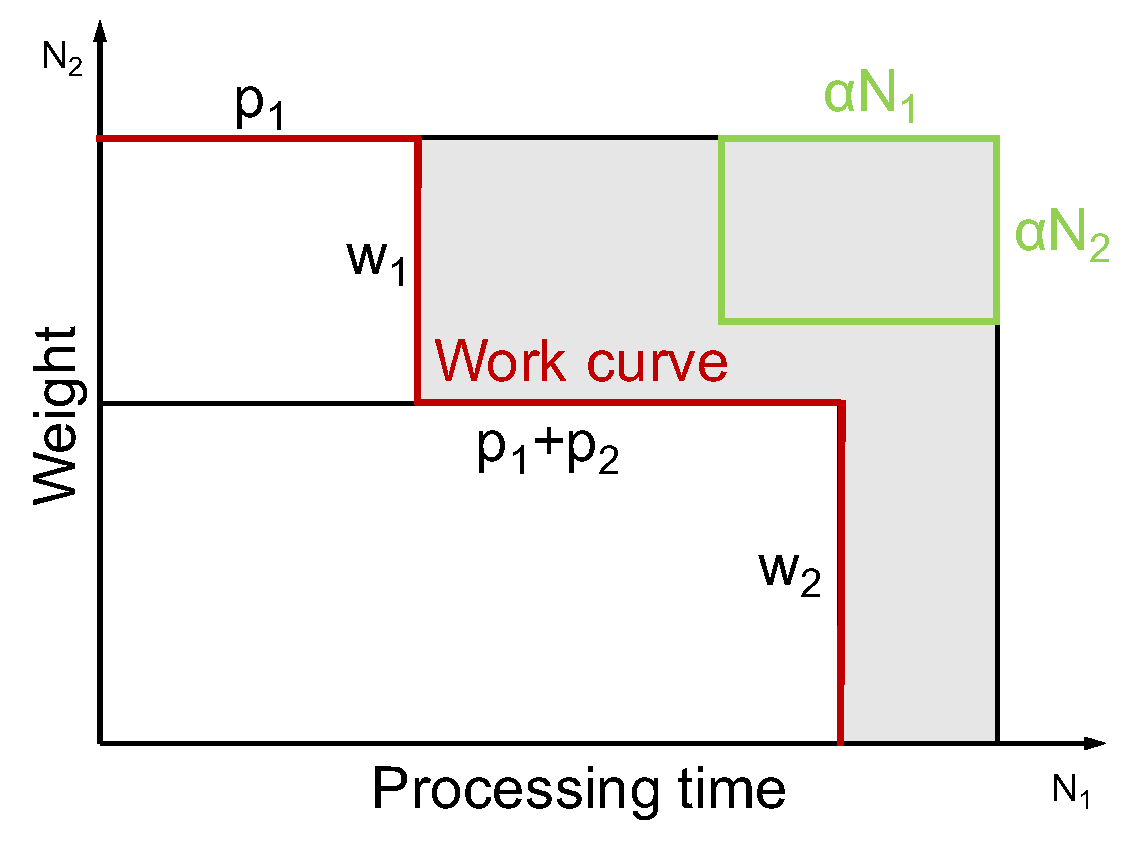
\includegraphics[width=0.5\textwidth]{figs/gantt.pdf}
	\caption{An example of 2D Gantt chart of a 0-1 bipartite instance.}
	\label{fig:gantt}
\end{figure}

The objective is to minimize the area under the work curve so as to minimize the sum of total weighted completion time. It turns out that the \emph{optimal} work curve has its area under the work curve very large for \emph{almost all} 0-1 bipartite instances. Since the weighted completion time is upper bounded by the total area (where every job finishes at largest time stamp) of the rectangular Gantt chart, the ``gap" between a feasible solution and the optimal solution is captured by the gray area in figure \ref{fig:gantt}.

We use an ancillary rectangle \emph{entirely} contained in the gray area, the green rectangle in figure \ref{fig:gantt} with $\alpha \in [0,1]$, to quantify the optimality gap and show that the area of this rectangle needs to be arbitrarily small with high probability when the number of machines $n$ is sufficiently large. 

For a desired fixed value $\alpha$, suppose the ancillary rectangle can fit in the gray area, there exists a set of $\lceil\alpha n_2\rceil$ jobs from $N_2$ that has at most $n_1 - \lceil\alpha n_1\rceil$ predecessors in $N_1$. In other words, if a rectangle of width $n_1$ and height $n_2$ can fit in the gray area, then there exists a set of $\lceil\alpha n_2\rceil$ jobs from $N_2$ and a set of $\lceil\alpha n_1\rceil$  jobs from $N_1$ with no precedence constraints between them.

Now suppose the way we construct the precedence constraint is that there is a fixed probability $q$ for each job in $N_1$ and $N_2$ to establish a precedence relation. Suppose we are given that the size $|N_1| = s$, and thus $|N_2| = n-s$, then the probability for there to be no precedence constraints between $N_1$ and $N_2$ is bounded by
\begin{align}
{s \choose \lceil\alpha s\rceil}{n-s \choose \lceil\alpha (n-s)\rceil}(1-q)^{ \lceil\alpha s\rceil \lceil\alpha (n-s)\rceil}. \label{eq:constructtwoclass}
\end{align}

Notice that the expoential term is over $(1-q)$ decays quickly to $0$ when $n$ is sufficiently large. The rest of the proof in \cite{schulz2011near} is essentially bounding the ${s \choose \lceil\alpha s\rceil}{n-s \choose \lceil\alpha (n-s)\rceil}$ term by forcing the distribution of $s$ to be ``balanced'' with high probability, meaning that the size of $n$ and $n-s$ should be within $\Theta(1)$. The details of the proof is omitted but the insight is that we want to construct the probability distribution $\pi_s$ for $s$, closed to ${n \choose 2} (1/2)^n$, for the size $s=0,1,..,n$. Then notice that ${s \choose \lceil\alpha s\rceil}{n-s \choose \lceil\alpha (n-s)\rceil}$ can be bounded by $2^n$ and thus the entire probability can be bounded by $O(n^2 (1-q)^{\alpha^2 s(n-s)})$, which goes to 0 when the number of jobs is sufficiently large. 